\documentclass[english,a4paper]{article}
%
\usepackage[a4paper]{geometry}
%\usepackage{fullpage}
\usepackage[T1]{fontenc}
\usepackage[latin9]{inputenc}
\usepackage{color}
\usepackage{graphicx}
\usepackage{babel}
%
\begin{document}

\section*{Figures}

\clearpage

\begin{figure}
\centering 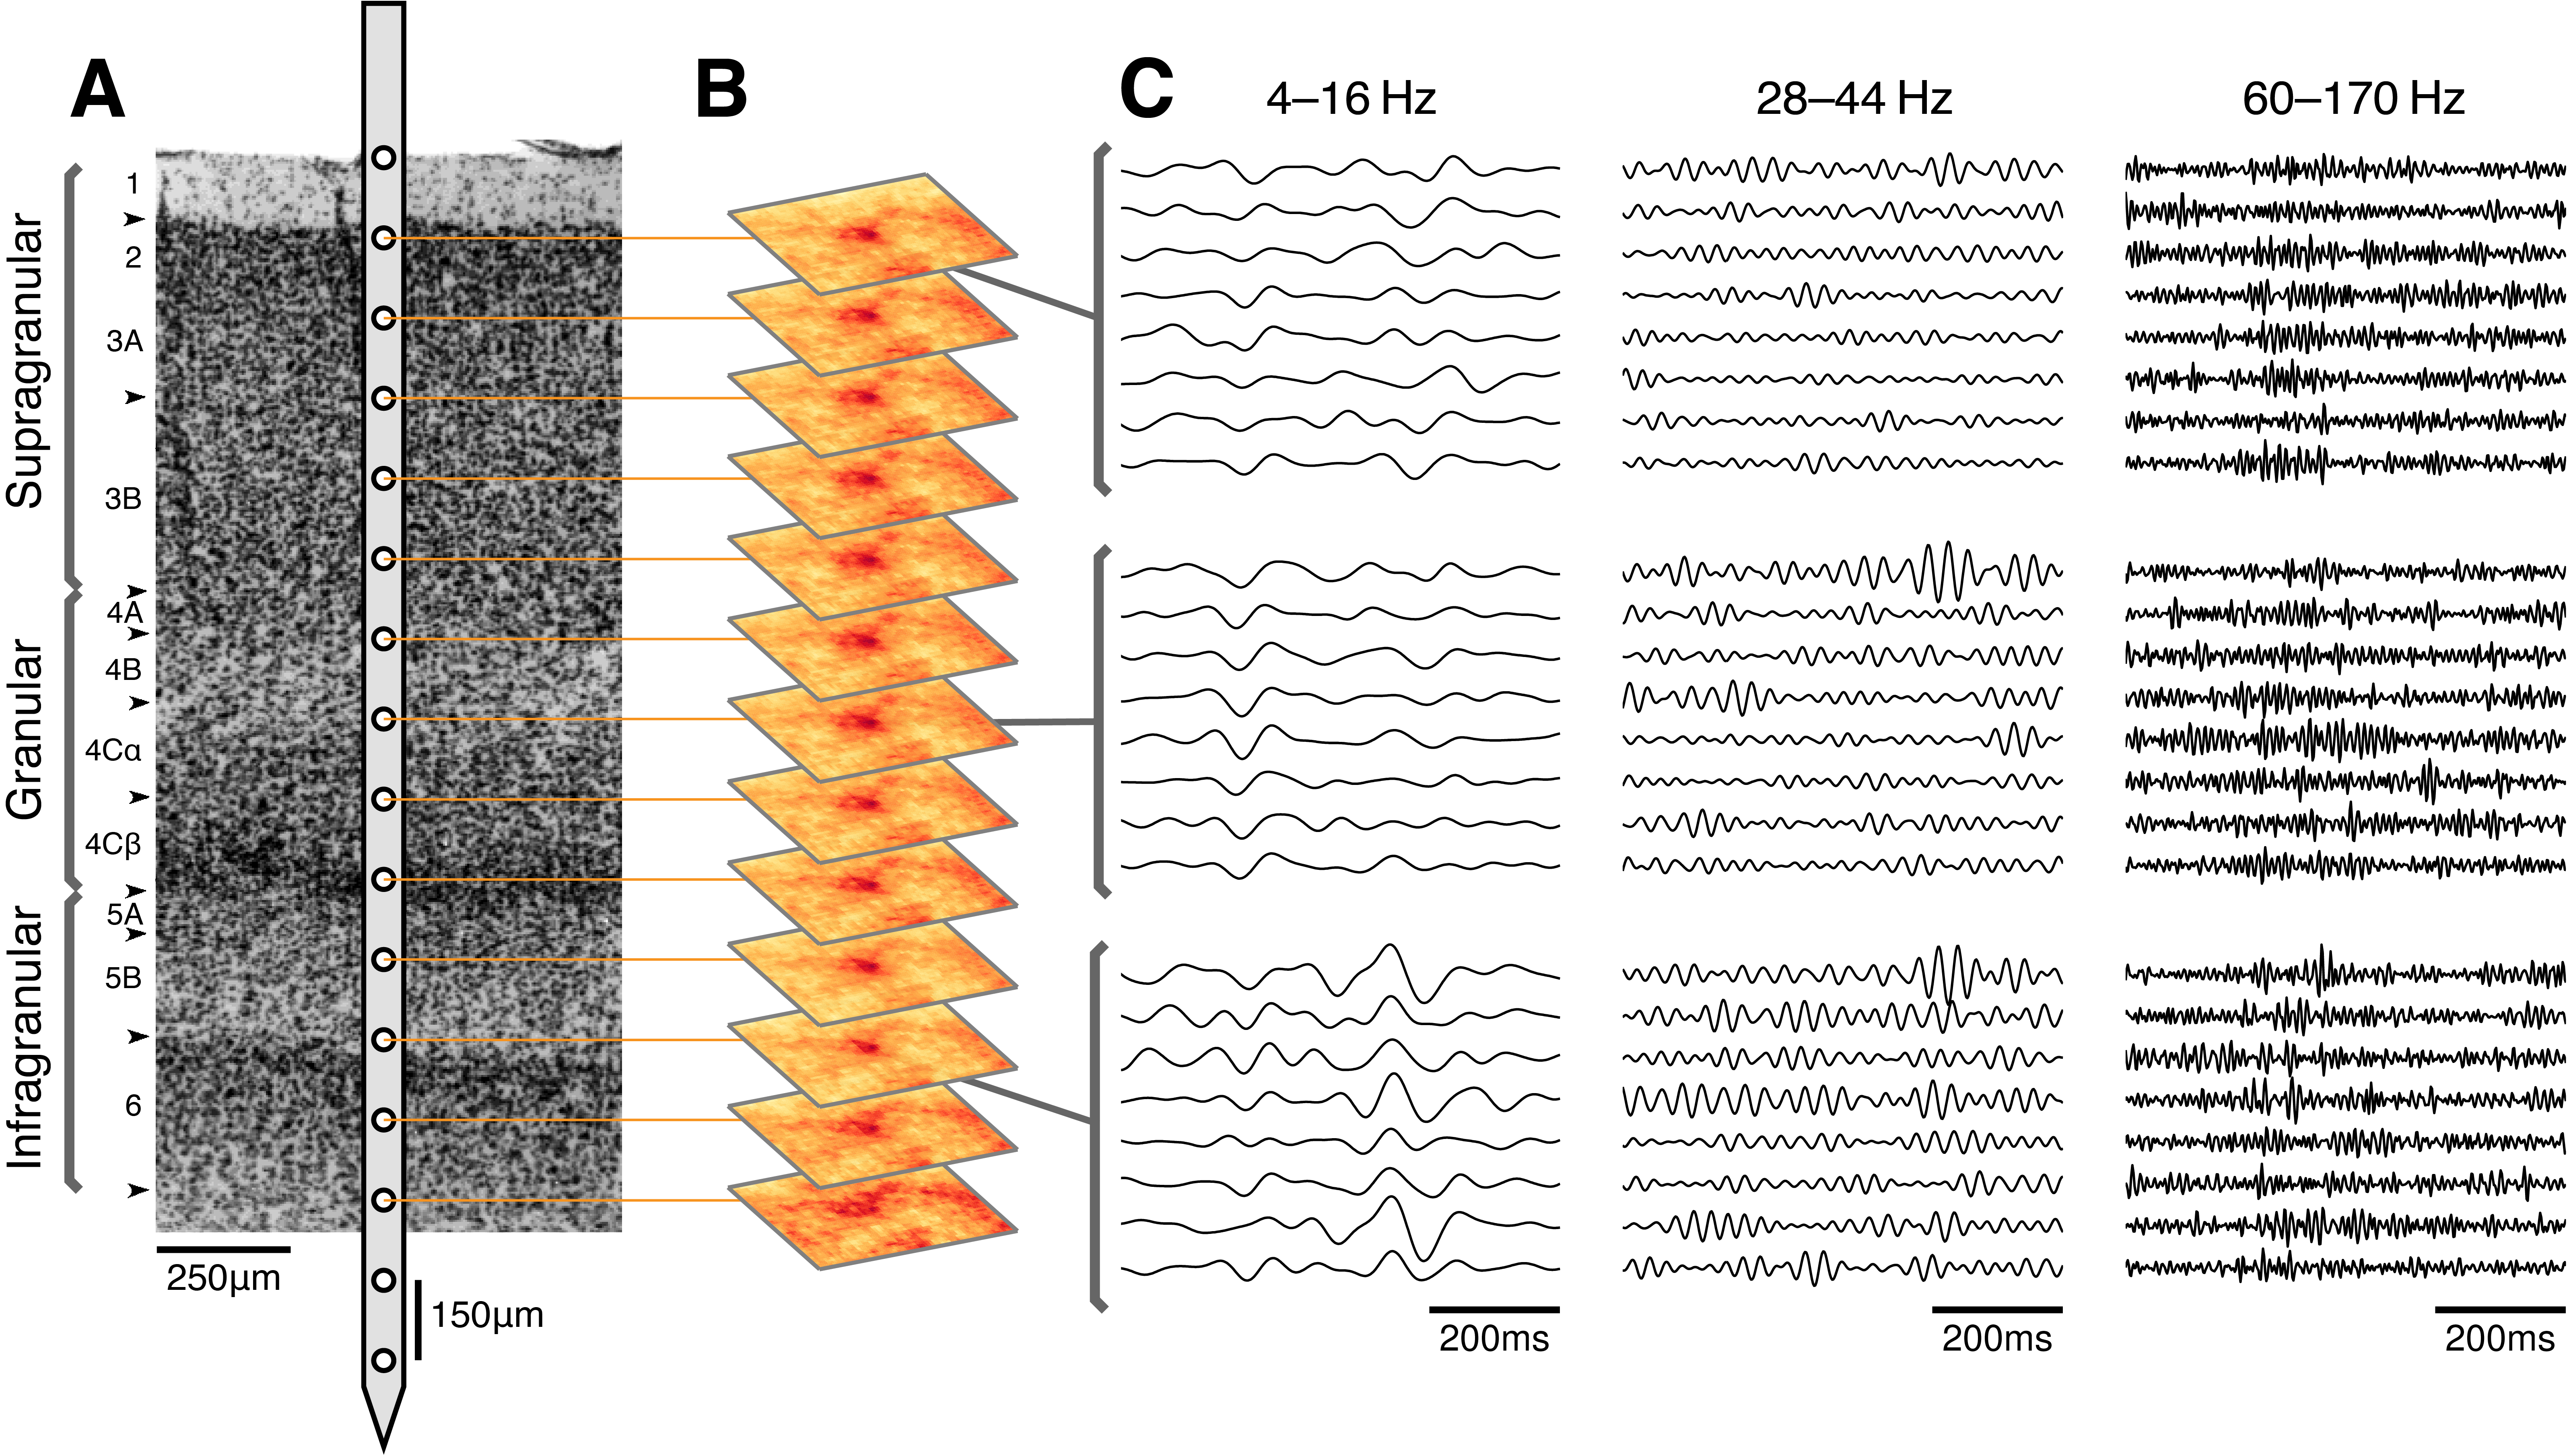
\includegraphics[width=\columnwidth]{fig1}
%
\caption{%
\textit{Overview of data collection and example data.}
A: Illustration of experimental recording setup, showing approximate locations 
of electrode contacts in relation to a Nissl-stained section of macaque V1 
cortex. Boundaries between cortical laminae are indicated with arrowheads. 
(Stain reproduced from Tyler et al. 1998, with permission.) (Note: Electrode 
width is not to scale.)
B: Receptive field locations were consistent across the 
cortical depth. Location of receptive field for each cortical recording site 
was identified by reverse 
correlating the multiunit activity (MUA) with the luminance changes of each 
pixel in the movie (session E07nm1).
C: Example CSD traces from simultaneous recordings at three cortical depths for eight 
repetitions of a movie fragment (session H05nm7).
The data are split into three temporal frequency bands (4-16Hz, 
28-44Hz and 60-170Hz, see Methods).
}
%
\end{figure}


\begin{figure}
\centering 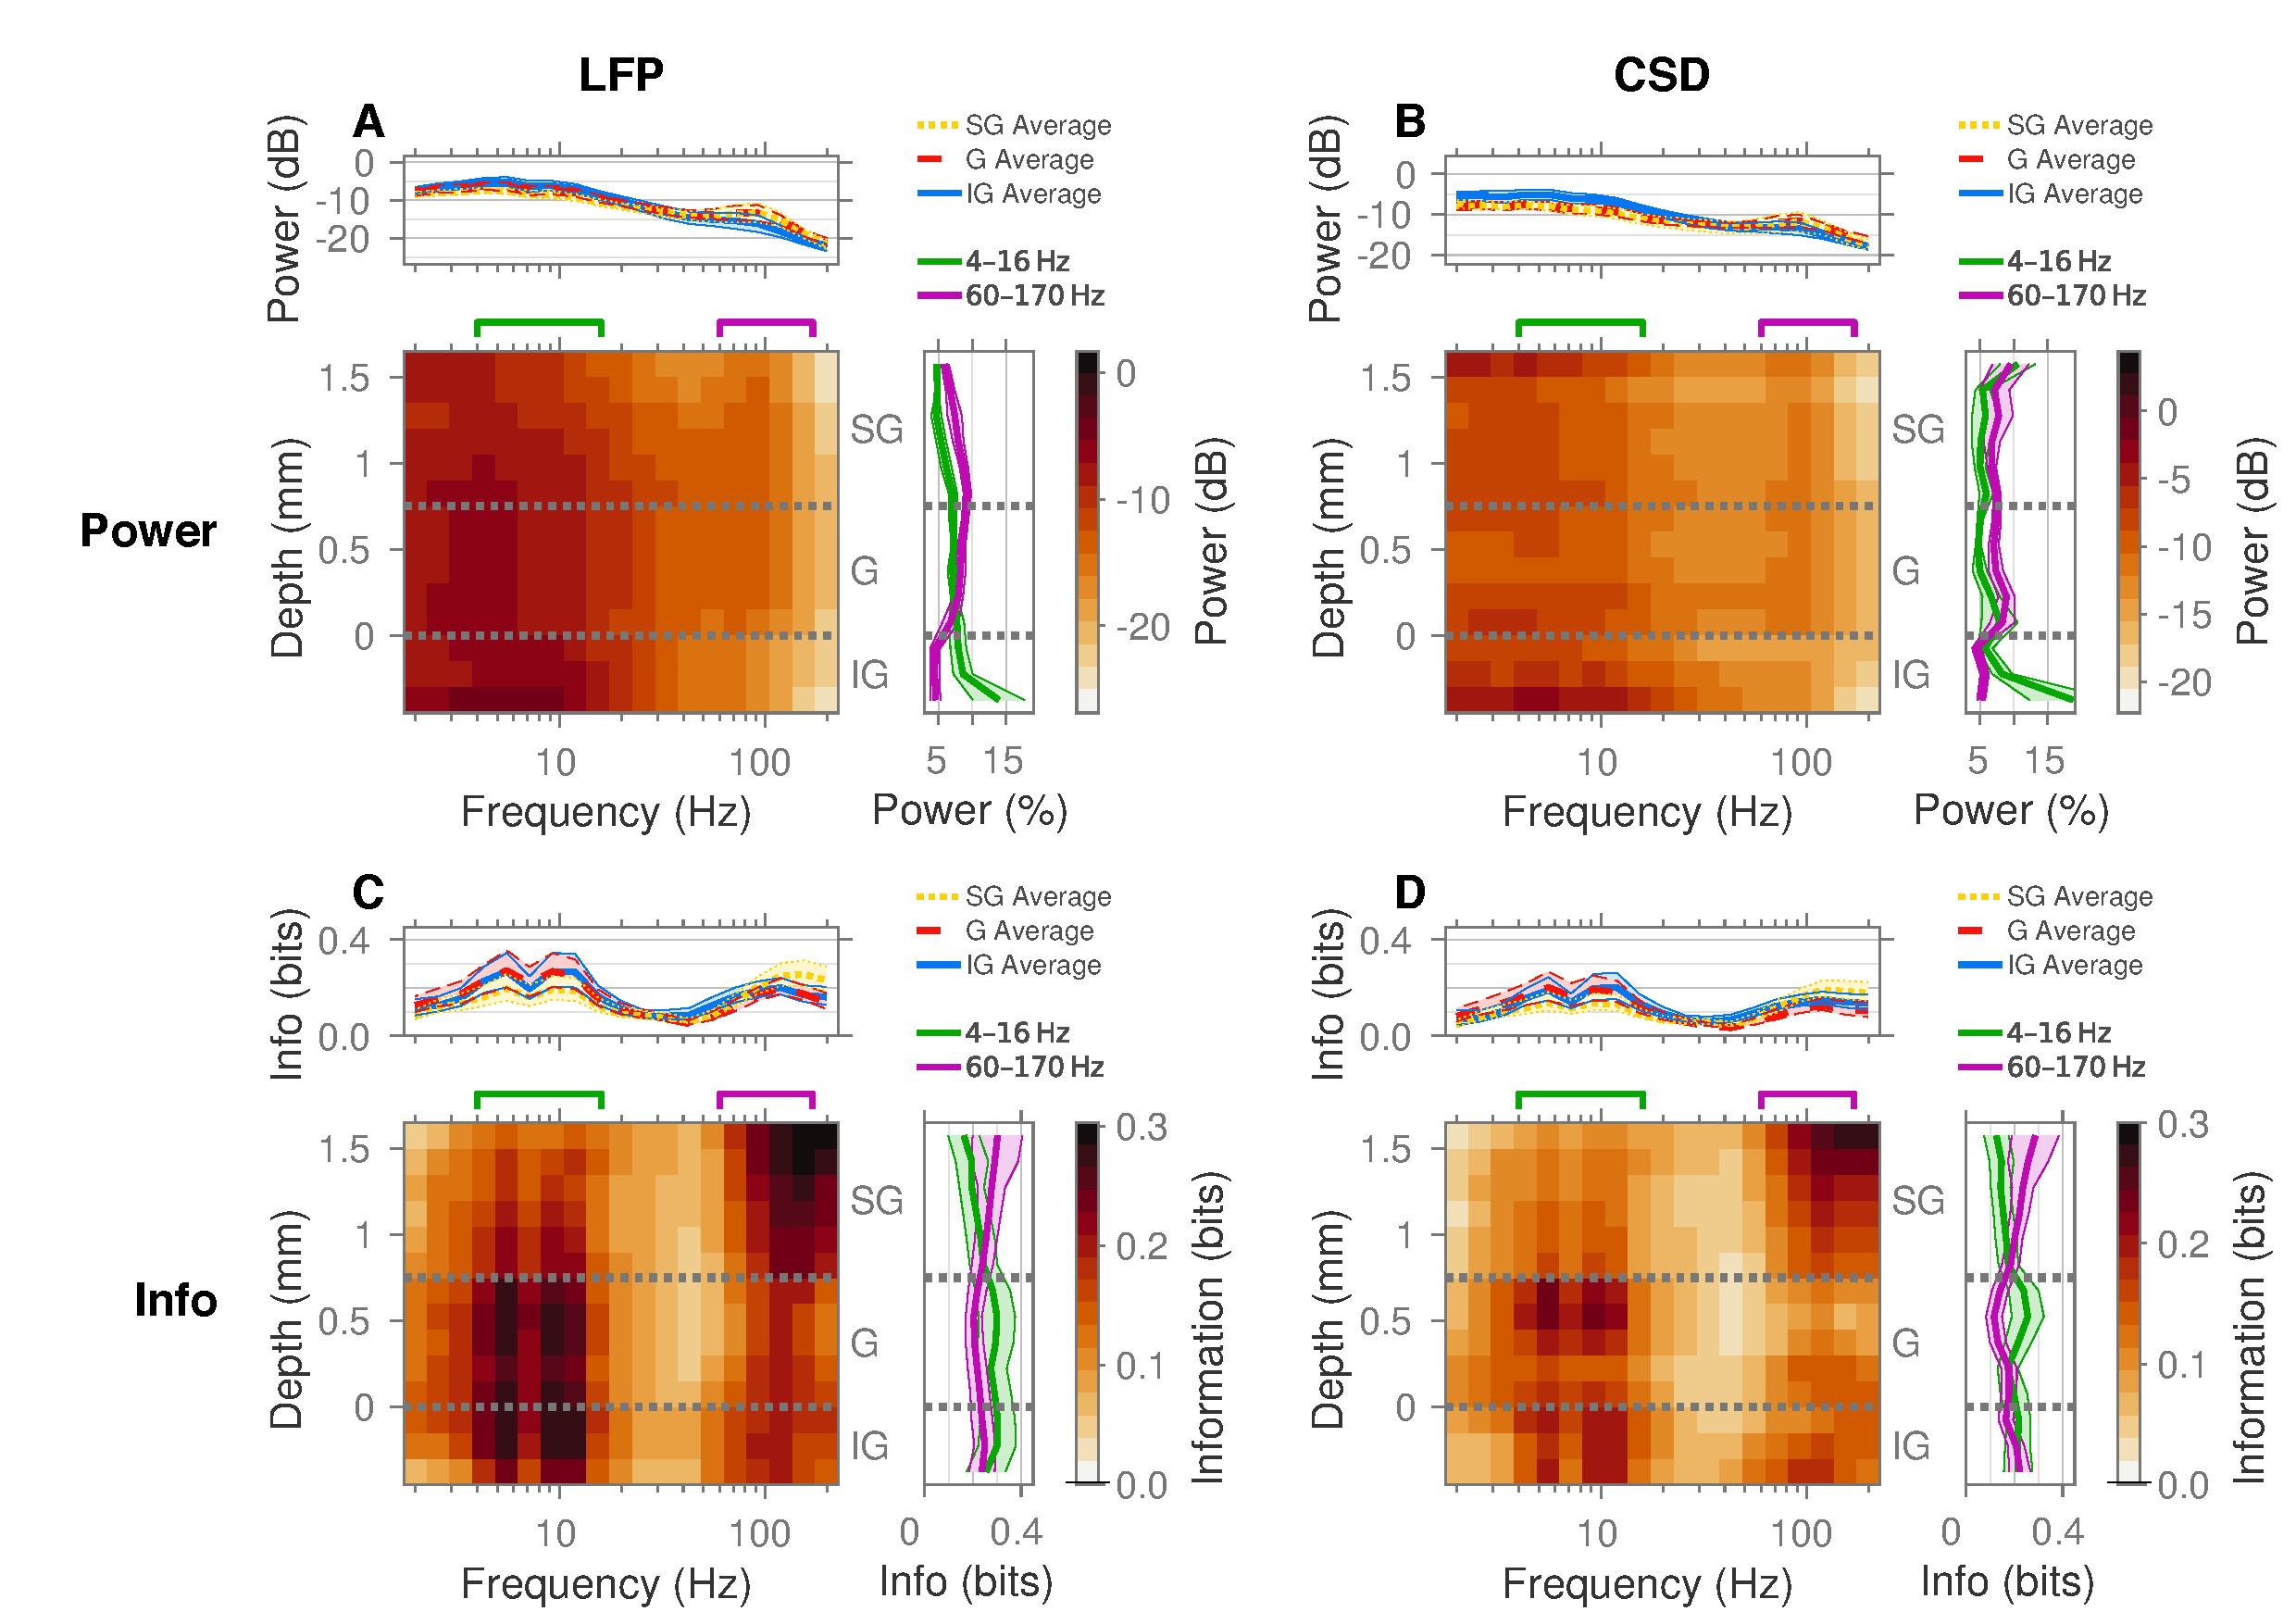
\includegraphics[width=\columnwidth]{fig2}
%
\caption{%
\textit{Distribution of visual stimulus information across both cortical depth 
and frequency.}
A: Distribution of LFP power during stimulus presentation. Plot shows the geometric mean 
power over 6 sessions. Above, mean power within supragranular (SG), granular 
(G) and infragranular (IG) regions. Right, laminar distribution of LFP power in
4-16Hz and 60-170Hz frequency bands.
B: Same as A, but distribution of CSD power instead of LFP power.
C: Distribution of information about the stimulus contained in LFP power. Plot 
shows the mean information over 6 sessions. Above, mean information within SG, G 
and IG regions. Right, cortical distribution of information in the power in
4-16Hz and 60-170Hz frequency bands.
D: Same as C, but for information in CSD power instead of LFP power.
Note that the information (C+D) is distributed very differently from the LFP and CSD power.
}
%
\end{figure}


\begin{figure}
\centering 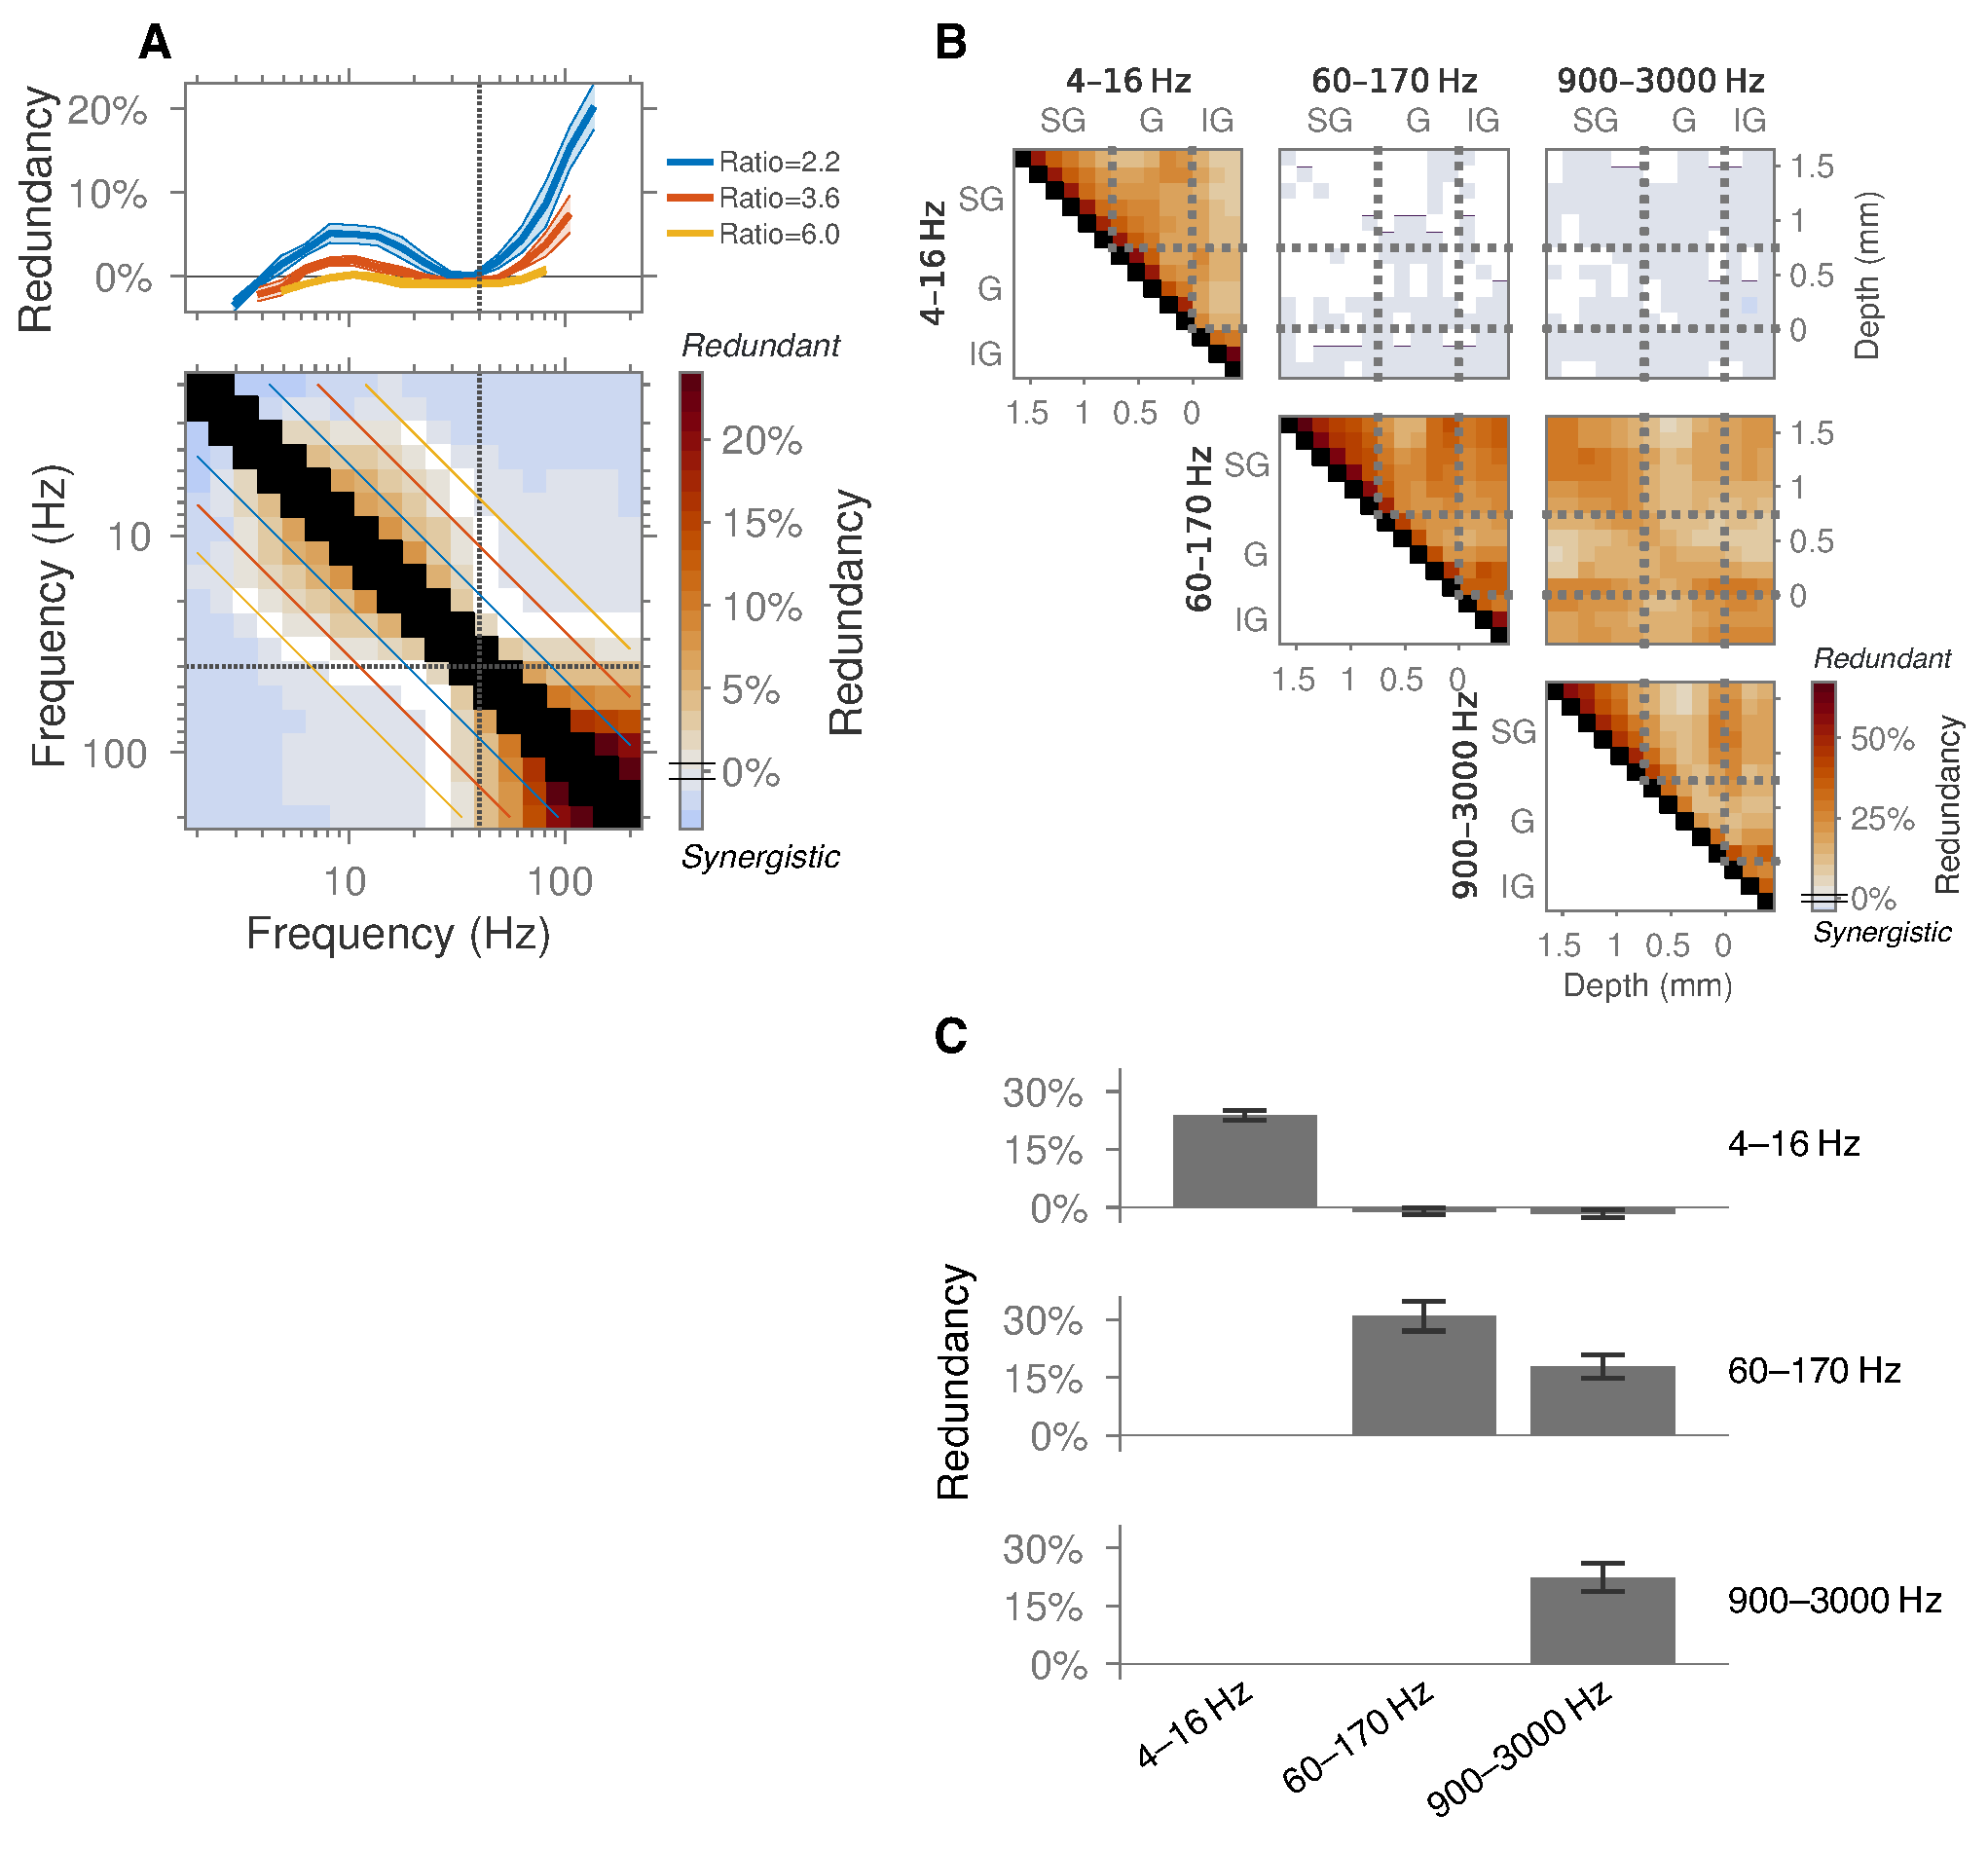
\includegraphics[width=\columnwidth]{fig3}
%
\caption{%
\textit{CSD information redundancy across frequency bands and laminae.}
A: Median redundancy between pairs of frequencies over the 12 recording 
sites, averaged over 6 sessions.
B: Redundancy between pairs of recording sites of the information in three 
frequency bands. Mean of 6 sessions.
C: Average of cross-channel redundancy shown in B.
Note, that while there is substantial redundancy within bands and between the 
60-170Hz and 900-3000Hz bands, there is little redundancy between the 4-16Hz and
60-170Hz band, indicating independent coding.
}
%
\end{figure}


\begin{figure}
\centering 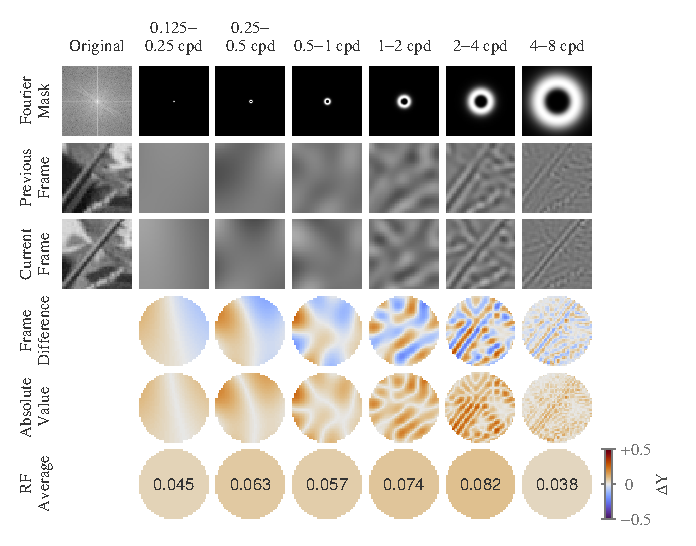
\includegraphics[width=\columnwidth]{fig4}
%
\caption{%
\textit{Extraction of spatially filtered luminance components.}
The luminance of the original video (left) is 
fast-Fourier transformed in a $224 \times 224$ px square for each frame (top-left: FFT of 
``current frame'').
The mask isolates bands of spatial frequencies that are one octave wide (Row 1), yielding 
the spatially filtered frames (Rows 2 and 3).
The stimulus magnitude at each spatial frequency band was obtained 
by taking the luminance difference of successive frames (Row 4), 
taking its absolute value (Row 5), 
and averaging this within the receptive field (Row 6).
%This provides us with a temporal sequence of the rate of change of luminance for 
%each spatial resolution.
}
%
\end{figure}


\begin{figure}
\centering 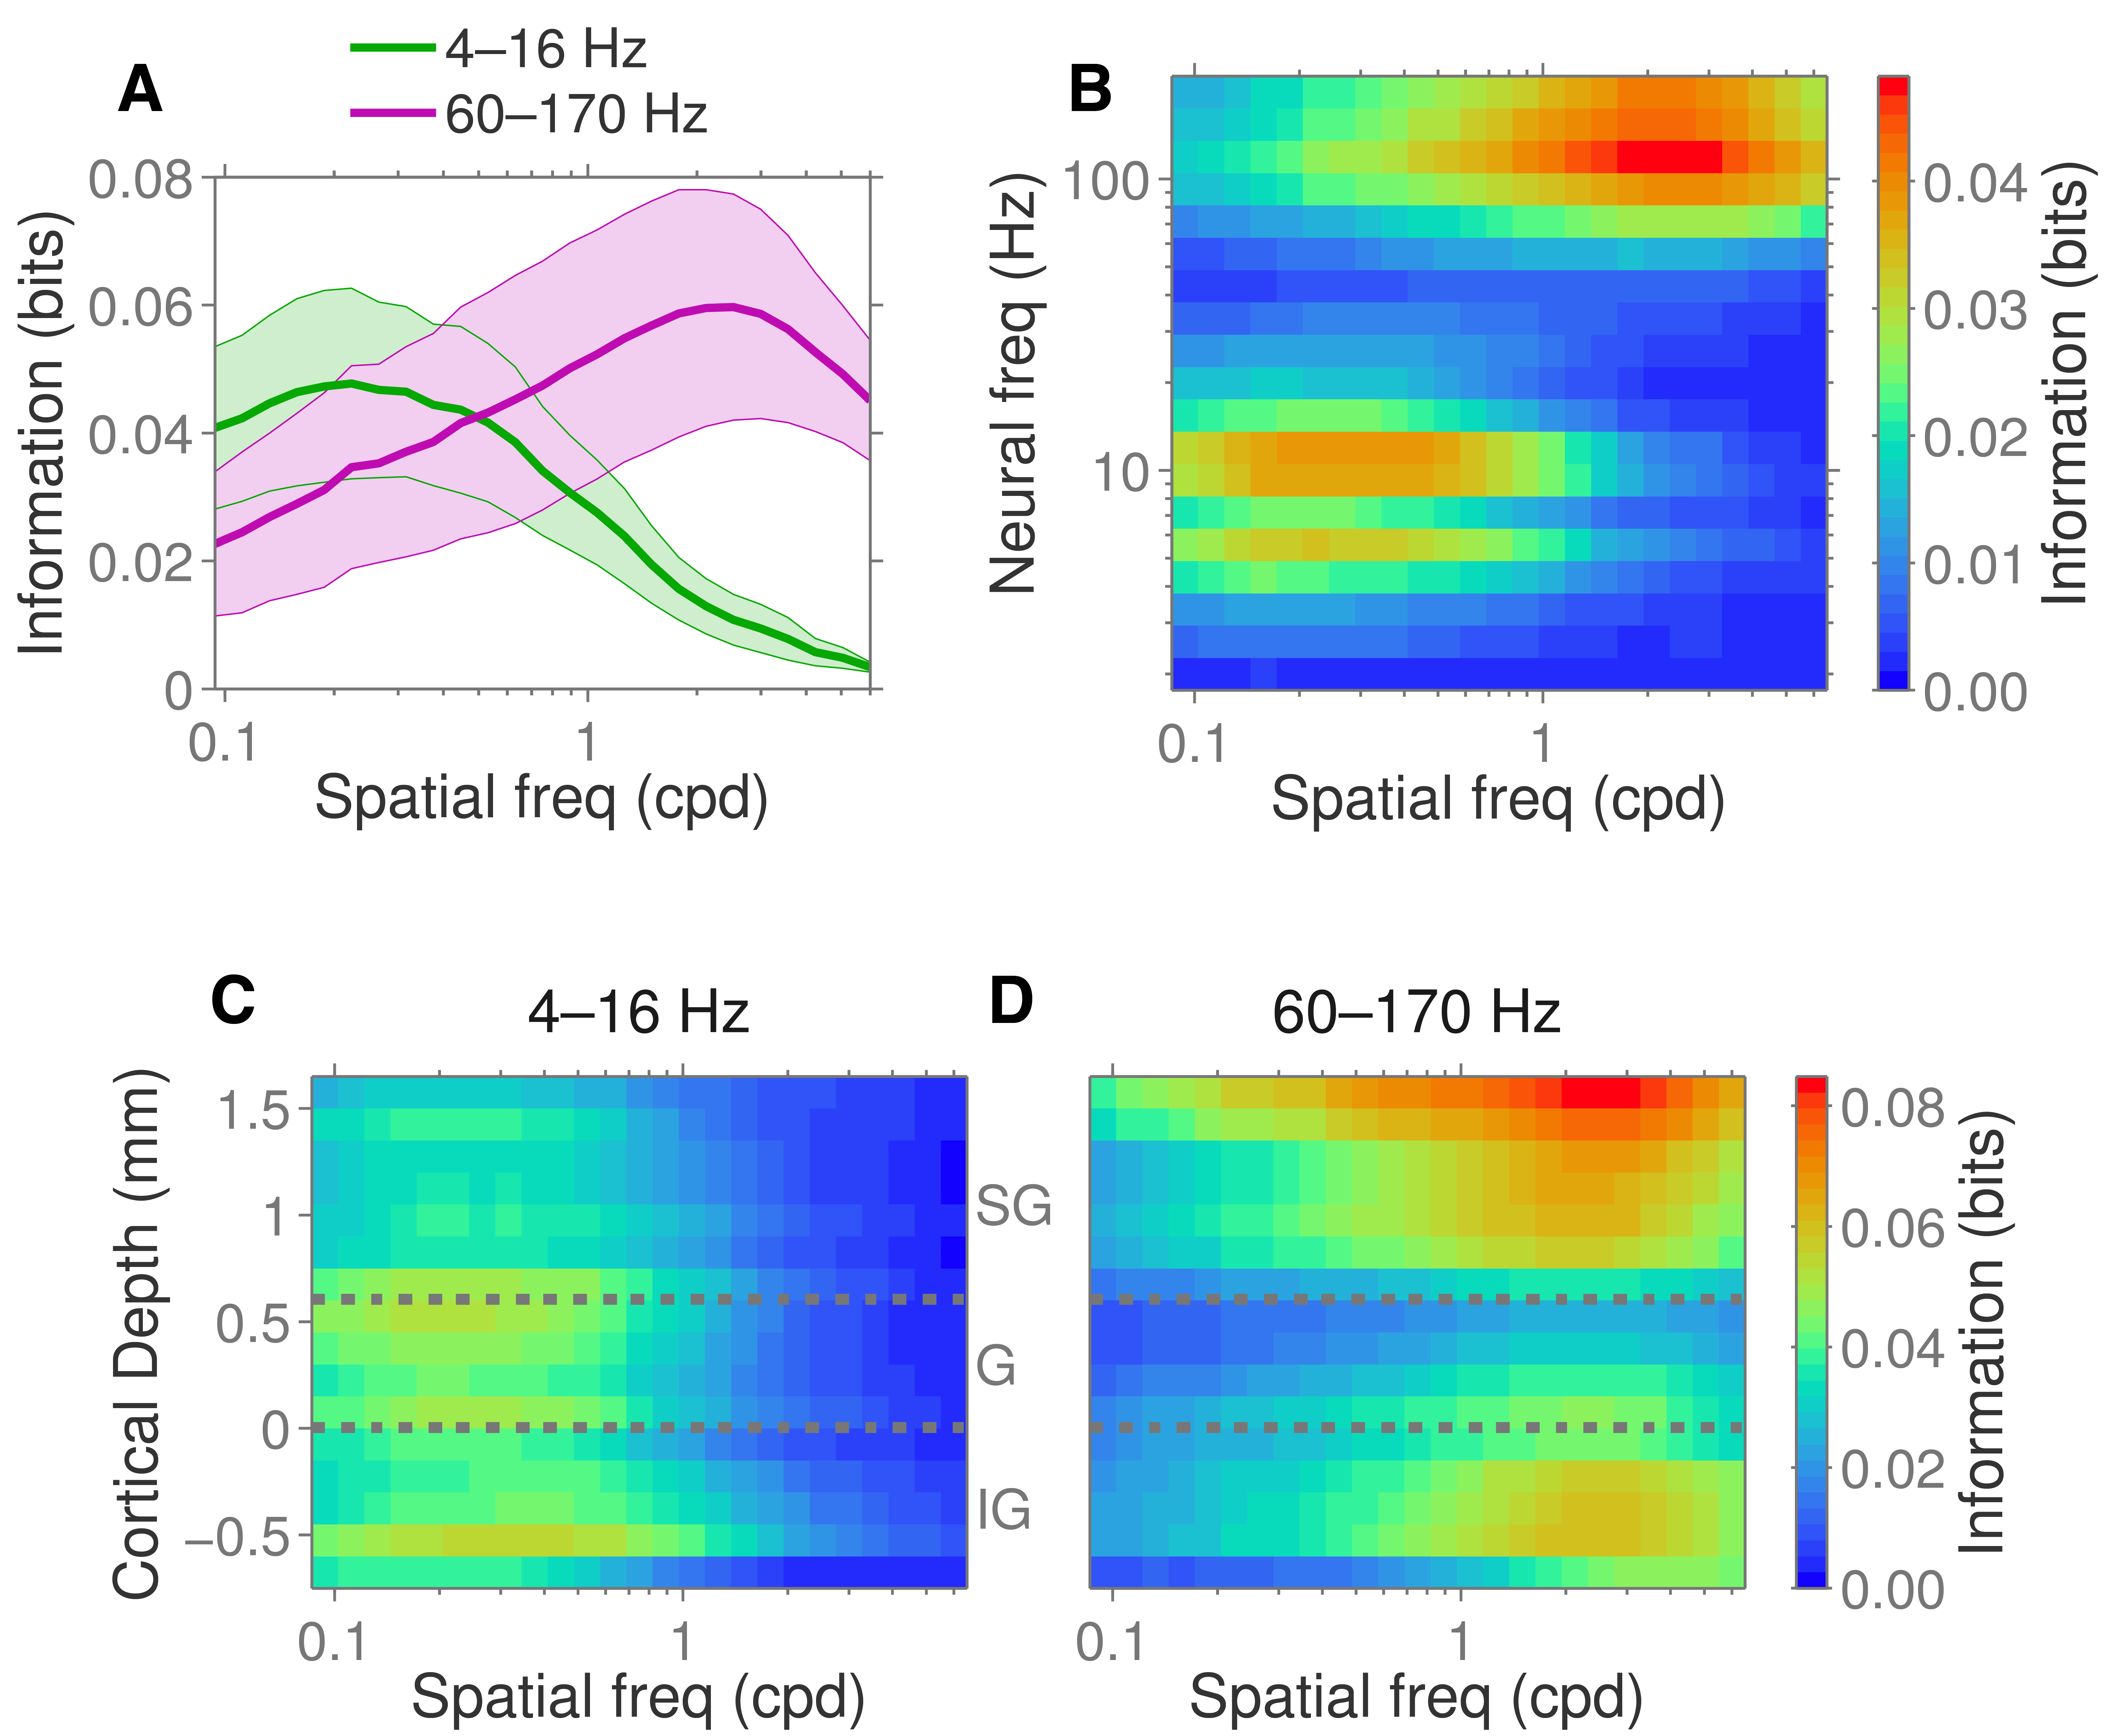
\includegraphics[width=\columnwidth]{fig5}
%
\caption{%
\textit{Information about different spatial components across laminae and frequency bands.}
A: Information about spatial components of the stimulus contained in 
low frequency CSD power (4-16Hz, average of information within G region; green) and high 
frequency CSD power (60-170Hz, average of information within SG region; purple). Shaded region: standard error across 6 sessions.
B: Information about visual spatial components contained in a range of CSD frequencies, median over 12 recording sites.
C,D: Information in low (4-16Hz) and high (60-170Hz) 
CSD frequency bands across cortical laminae.
Plots A-D are mean of 6 sessions.
}
%
\end{figure}


\begin{figure}
\centering 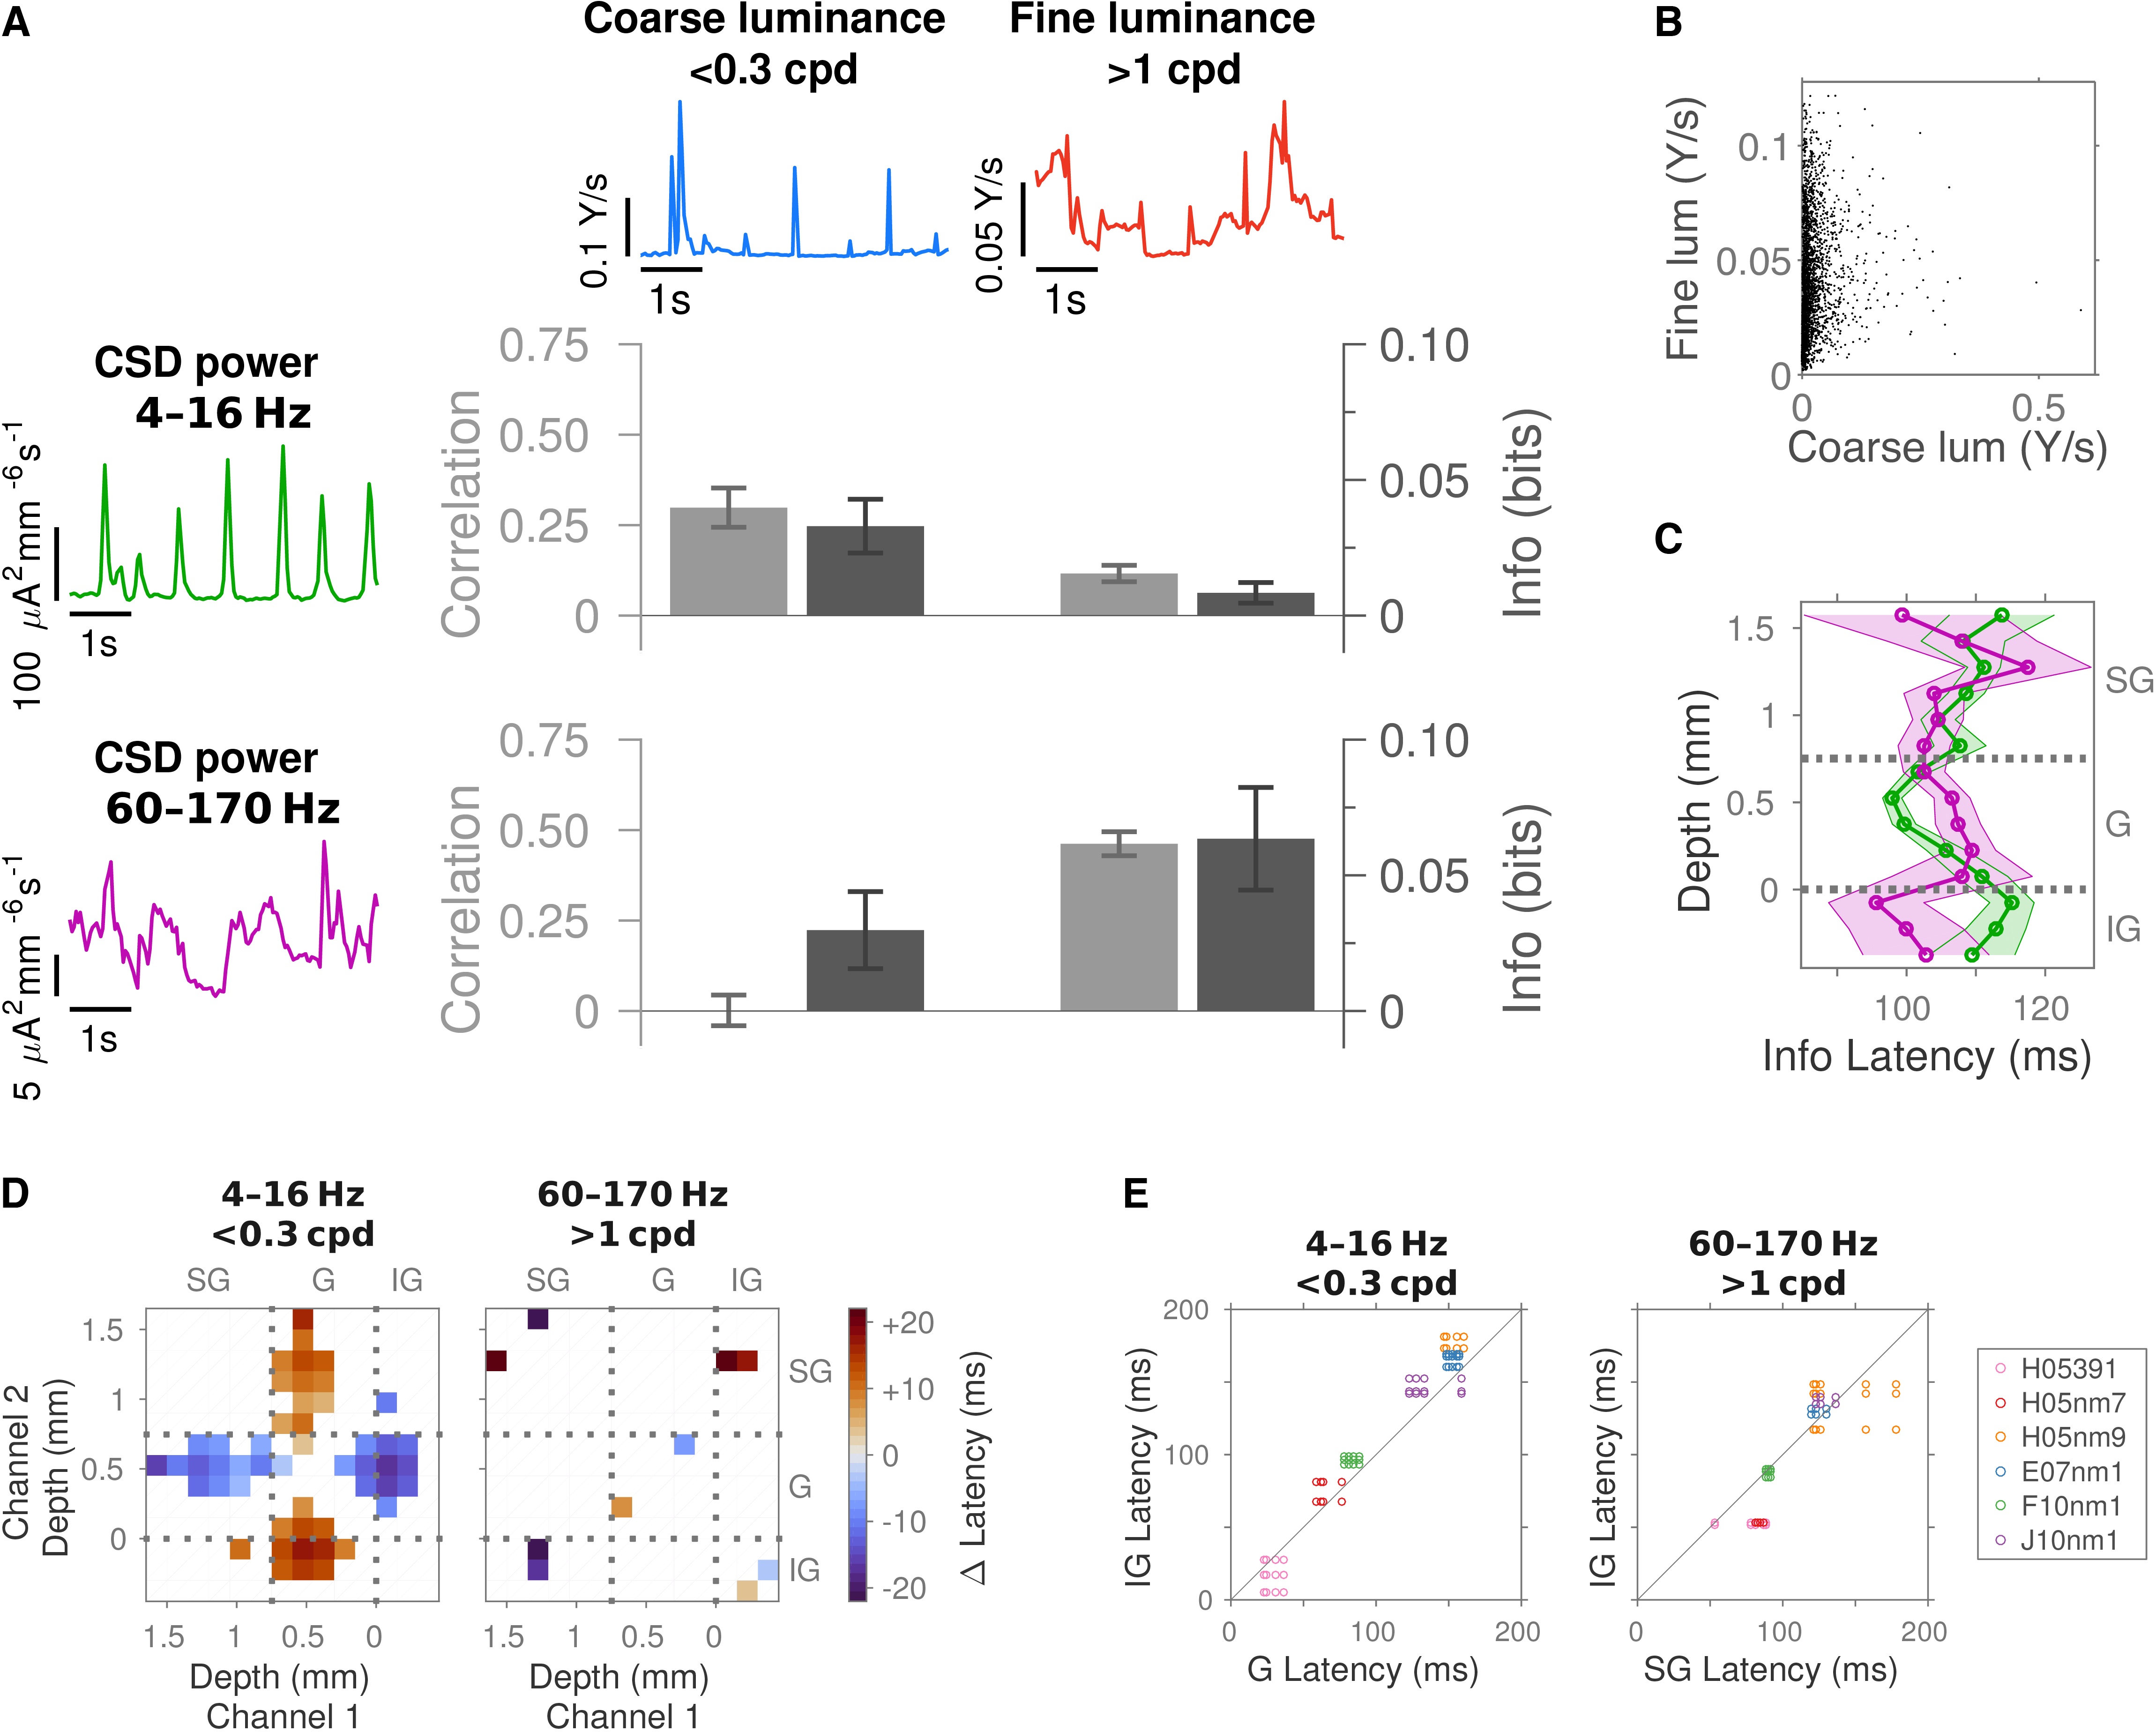
\includegraphics[width=\columnwidth]{fig6}
%
\caption{%
\textit{Overview of information components.}
A: Relationship between Coarse/Fine changes in luminance and Low/High frequency neural activity.
Left: Instantaneous power in 4-16Hz band (averaged over trials and SG layers) and 60-170Hz band (averaged over trials and G layers) for an example session (H05nm7).
Above: Coarse (<0.3cpd) and fine (>1cpd) rate of change in luminance over the same time period.
The barchart shows, for each pair of stimulus and response, Pearson's correlation coefficient (pale grey; left-hand axis) and mutual information (dark grey; right-hand axis).
B: Fine versus coarse change in luminance for each frame change in the stimulus.
C: Lag between stimulus and response yielding maximal information (green: 4-16Hz and coarse luminance; purple: 60-170Hz and fine luminance).
}
%
\end{figure}



\begin{figure}
\centering 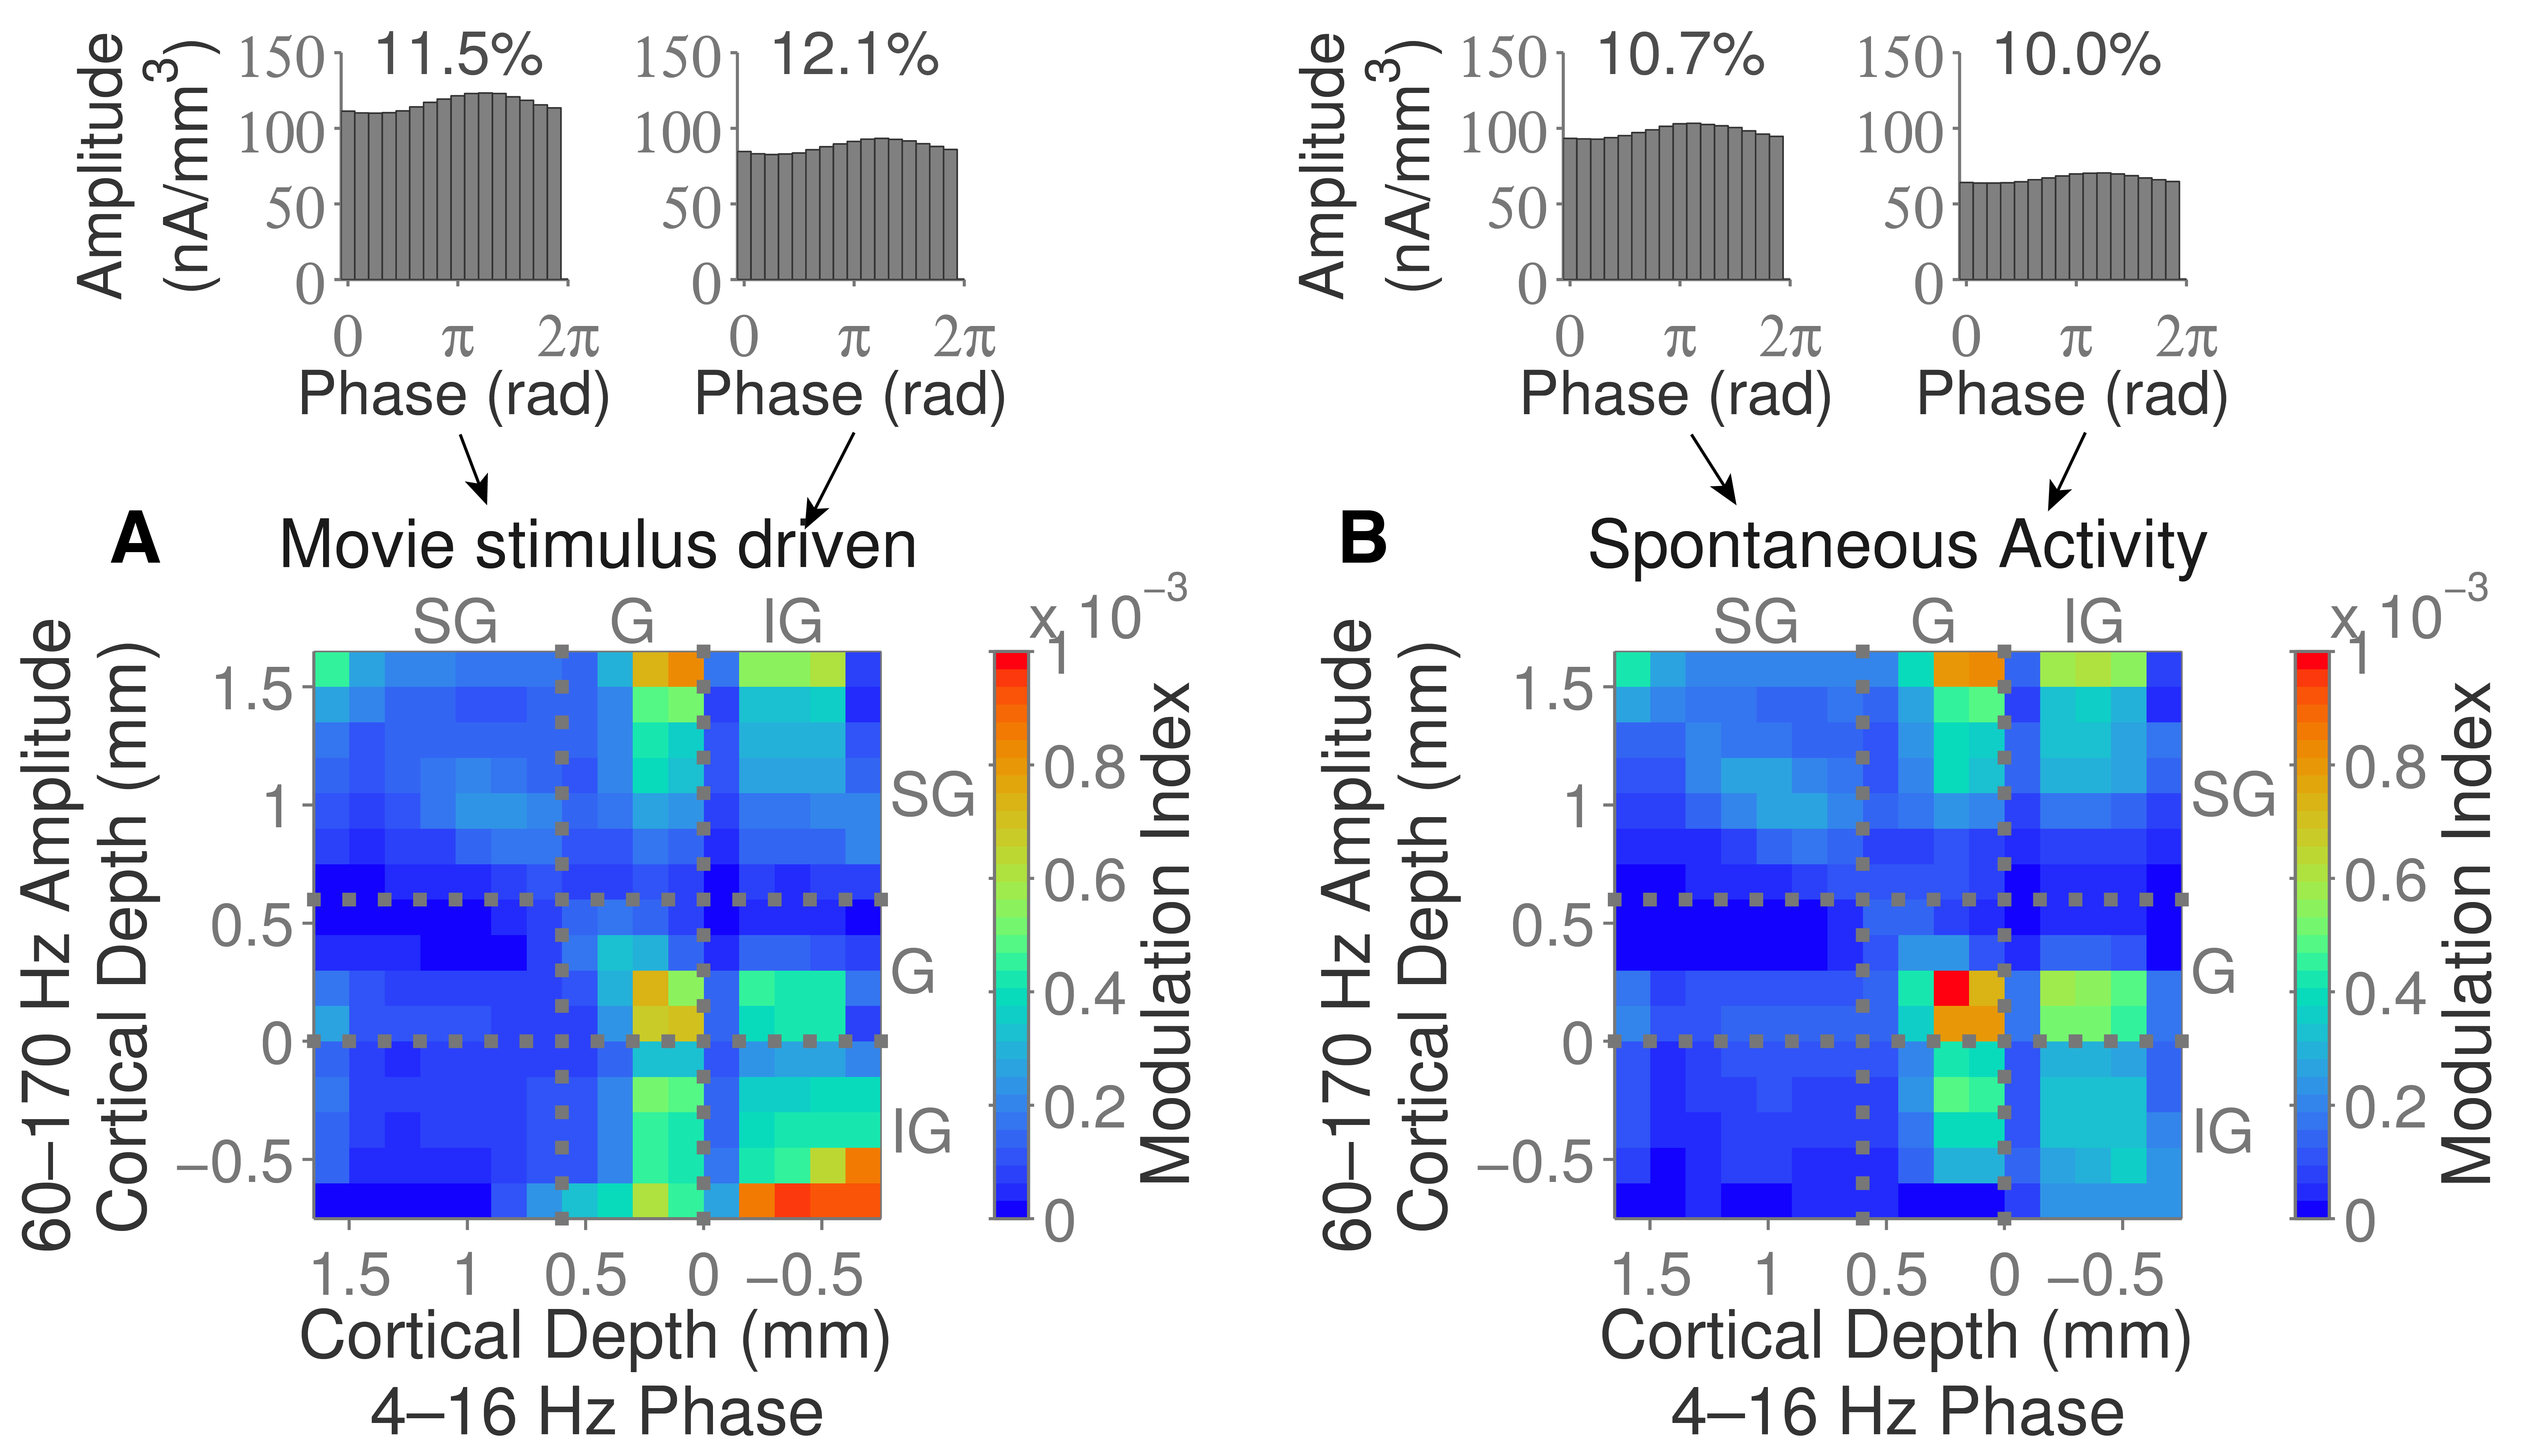
\includegraphics[width=\columnwidth]{fig8}
%
\caption{%
\textit{Cross-frequency phase-amplitude coupling}
Phase-amplitude modulation index between low frequency (4-16Hz) phase and high 
frequency (60-170Hz) amplitude (A: movie driven activity; B: spontaneous 
activity). Mean of 5 sessions.
Above, amplitude as a function of binned phase for an example session (H05391). 
Left inset: IG/IG coupling; Right inset: IG/SG coupling.
}
%
\end{figure}



\end{document}